\documentclass[11pt,a4paper]{article}
\usepackage{fontspec}
\setmainfont[Path=fonts/,FontIndex=7,BoldFont=AvenirNext.ttc,BoldFeatures={FontIndex=2},ItalicFont=AvenirNext.ttc,ItalicFeatures={FontIndex=4},BoldItalicFont=AvenirNext.ttc,BoldItalicFeatures={FontIndex=3}]{AvenirNext.ttc}
\setsansfont[Path=fonts/,FontIndex=7,BoldFont=AvenirNext.ttc,BoldFeatures={FontIndex=2},ItalicFont=AvenirNext.ttc,ItalicFeatures={FontIndex=4},BoldItalicFont=AvenirNext.ttc,BoldItalicFeatures={FontIndex=3}]{AvenirNext.ttc}
\newfontfamily\heavy[Path=fonts/,FontIndex=2]{AvenirNext.ttc}
\setmonofont[Path=fonts/,BoldFont=JetBrainsMono-Bold.ttf,ItalicFont=JetBrainsMono-Italic.ttf,Contextuals=NoAlternate,Ligatures=NoCommon]{JetBrainsMono-Regular.ttf}
\usepackage{xcolor,graphicx,tikz,booktabs,tabularx,listings,amsmath}
\usetikzlibrary{arrows.meta,positioning}
\definecolor{paper}{HTML}{FFFFFF}
\definecolor{ink}{HTML}{252525}
\definecolor{teal}{HTML}{252525}
\definecolor{orange}{HTML}{777777}
\definecolor{wash}{HTML}{EAEAEA}
\definecolor{quiet}{HTML}{666666}
\definecolor{lightink}{HTML}{D0D0D0}
\definecolor{codepaper}{HTML}{F6F6F4}
\lstset{language=Python,basicstyle=\ttfamily\fontsize{9.5}{13}\selectfont\color{ink},keywordstyle=\bfseries\color{ink},commentstyle=\itshape\color{quiet},stringstyle=\color{ink},showstringspaces=false,columns=fullflexible,keepspaces=true,breaklines=true,breakatwhitespace=true,numbers=none,upquote=true,aboveskip=8pt,belowskip=6pt}
\hyphenpenalty=4000
\emergencystretch=3em
% The same two-line navigation and fine rule as the reference, without a candy motif.
\newcommand{\guideheader}[2]{\begin{tikzpicture}[remember picture,overlay]
\node[anchor=north west,inner sep=0,text width=176mm] at ([xshift=16mm,yshift=-7mm]current page.north west) {\fontsize{8.5}{10}\selectfont\color{quiet}#1};
\node[anchor=north west,inner sep=0,text width=176mm] at ([xshift=16mm,yshift=-11.5mm]current page.north west) {\heavy\fontsize{10}{12}\selectfont\color{ink}#2};
\draw[lightink,line width=.4pt] ([xshift=16mm,yshift=-17mm]current page.north west)--([xshift=192mm,yshift=-17mm]current page.north west);
\end{tikzpicture}}

\usepackage[a4paper,left=16mm,right=18mm,top=24mm,bottom=19mm,headheight=14pt]{geometry}
\usepackage{fancyhdr,enumitem,hyperref}
\hypersetup{colorlinks=true,linkcolor=teal,urlcolor=teal}
\setlength{\parindent}{0pt}
\setlength{\parskip}{7pt}
\setlist{nosep,leftmargin=1.4em}
\usepackage{needspace,colortbl}
\lstdefinestyle{numbered}{numbers=left,numberstyle=\ttfamily\fontsize{7.5}{13}\selectfont\color{lightink},numbersep=10pt,xleftmargin=24pt}
\pagestyle{fancy}\fancyhf{}
\fancyhead[C]{\guideheader{Lesson 3 · Mortal Kombat Tower and Array Description}{Worksheet Answers · \nouppercase{\leftmark}}}
\fancyfoot[L]{\fontsize{8}{10}\selectfont\color{quiet}LESSON 3 / Mortal Kombat Tower and Array Description}
\fancyfoot[R]{\fontsize{9}{11}\selectfont\color{quiet}\thepage}
\renewcommand{\headrulewidth}{0pt}
\newcommand{\topic}[2]{\clearpage\markboth{#2}{}{\color{quiet}\fontsize{9}{12}\selectfont\textbf{#1}}\par{\heavy\fontsize{19}{23}\selectfont\raggedright #2\par}\vspace{5pt}}
\newcommand{\topicflow}[2]{\par\Needspace{20\baselineskip}\bigskip\markboth{#2}{}{\color{quiet}\fontsize{9}{12}\selectfont\textbf{#1}}\par{\heavy\fontsize{19}{23}\selectfont\raggedright #2\par}\vspace{5pt}}
\newcommand{\labeltext}[1]{{\color{teal}\textbf{#1}}\par}
\makeatletter
\newsavebox{\qbox}
\newenvironment{qblock}[1][0.6]{\def\qlimit{#1}\par\setbox\qbox\vbox\bgroup\hsize\linewidth\color@begingroup}{\par\color@endgroup\egroup
  \ifdim\dimexpr\ht\qbox+\dp\qbox\relax>\qlimit\textheight\relax\unvbox\qbox\else\box\qbox\fi\par}
\makeatother
\newcommand{\qtopic}[2]{{\color{quiet}\fontsize{9}{12}\selectfont\textbf{#1}}\par{\heavy\fontsize{19}{23}\selectfont\raggedright #2\par}\vspace{5pt}}
\begin{document}\color{ink}\fontsize{10.5}{13}\selectfont
\thispagestyle{empty}\pagecolor{white}\null
\begin{tikzpicture}[remember picture,overlay]
\node[anchor=north west,inner sep=0,text width=174mm] at ([xshift=18mm,yshift=-22mm]current page.north west)
{\heavy\fontsize{9}{12}\selectfont ALGORITHMS\quad /\quad LESSON 03\quad /\quad WORKSHEET ANSWERS};
\node[anchor=north west,inner sep=0,text width=174mm] at ([xshift=18mm,yshift=-39mm]current page.north west)
{\heavy\fontsize{33}{37}\selectfont\raggedright\spaceskip=.25em Mortal Kombat Tower\\and Array Description\par};
\node[anchor=north west,inner sep=0,text width=174mm] at ([xshift=18mm,yshift=-80mm]current page.north west)
{\fontsize{19}{25}\selectfont Worked answers, tables and complete code.};
\node[anchor=north west,inner sep=0,text width=150mm] at ([xshift=18mm,yshift=-97mm]current page.north west)
{\fontsize{12}{16}\selectfont Check each answer against your own working.\\Follow the question IDs from the worksheet.};
\node[anchor=center,inner sep=0] at ([xshift=105mm,yshift=-167mm]current page.north west)
{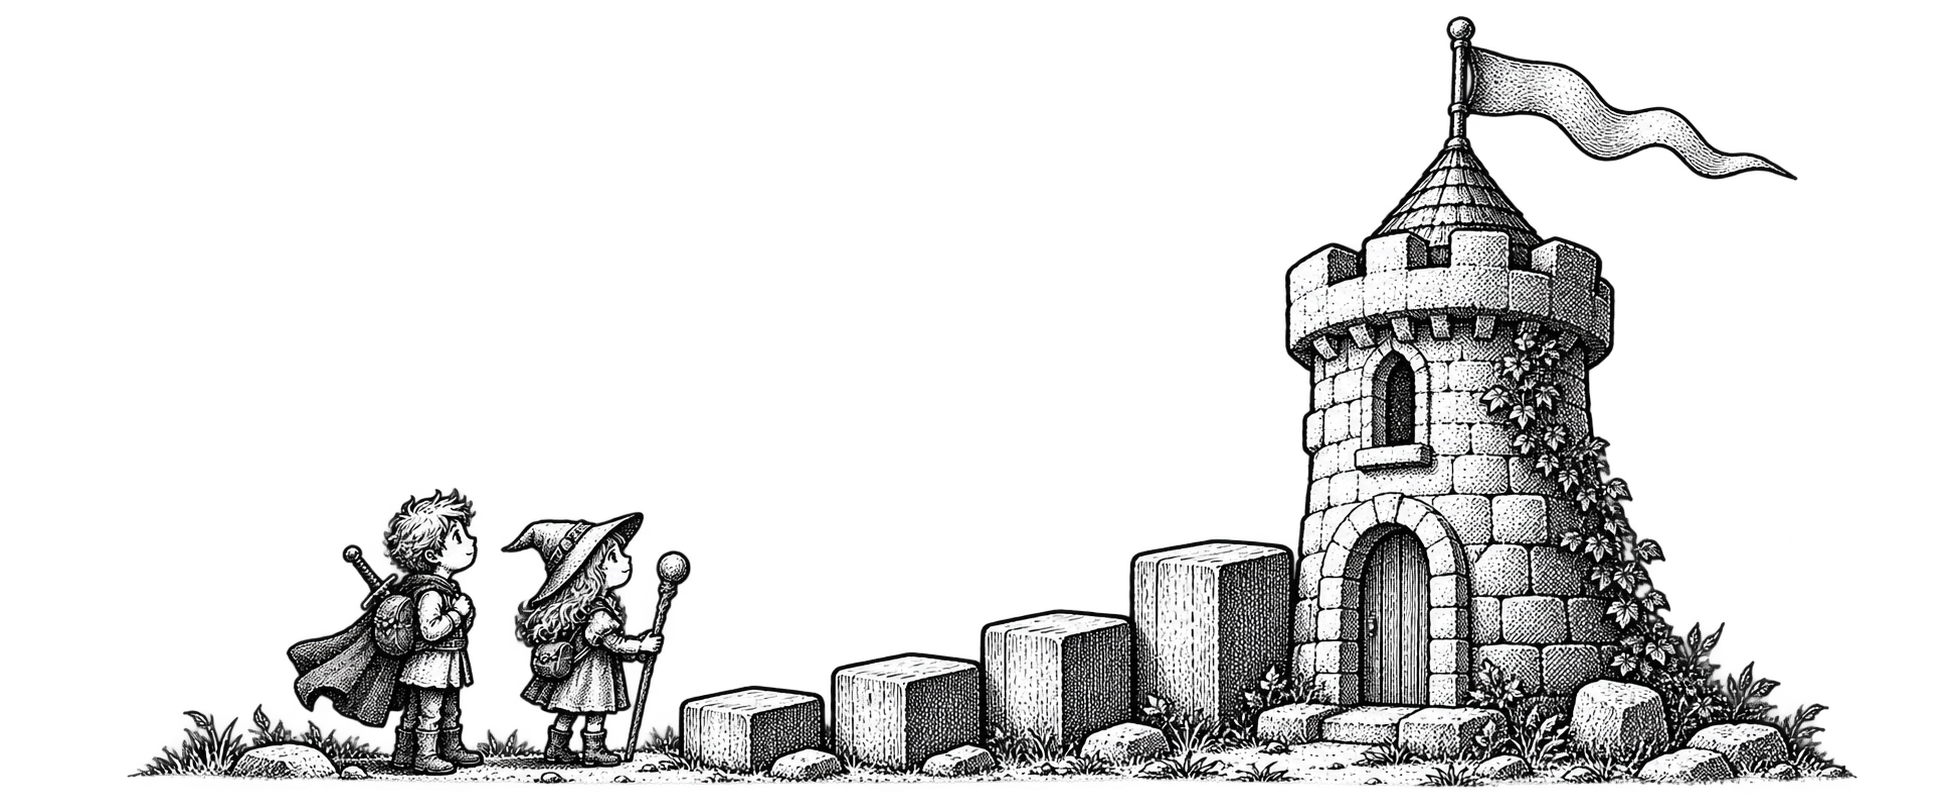
\includegraphics[width=174mm,height=94mm,keepaspectratio]{assets/cover.png}};
\node[anchor=north west,inner sep=0,text width=174mm] at ([xshift=18mm,yshift=-224mm]current page.north west)
{\fontsize{12}{16}\selectfont Questions appear in worksheet order.\\Alternative correct solutions are welcome.};
\node[anchor=west,inner sep=0] at ([xshift=18mm,yshift=-269mm]current page.north west)
{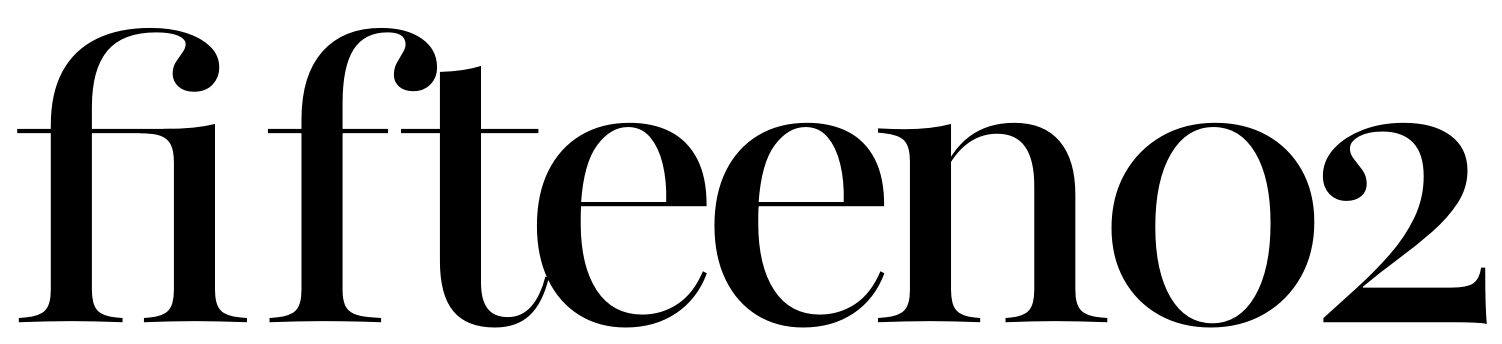
\includegraphics[width=43mm]{assets/logo.png}};
\node[anchor=east,inner sep=0] at ([xshift=192mm,yshift=-269mm]current page.north west)
{
\includegraphics[width=62mm]{assets/julians-pathfinder-monochrome.pdf}};
\end{tikzpicture}\clearpage
\topic{KEEP BESIDE YOUR WORK}{The route and the rules}
\textbf{Our route}\par Ask what extra information changes the available choices. Tower needs the next player as well as the boss position. Array Description needs the neighbouring value as well as the position. Work a small case, describe the stored answer, then write recursion and a table.\par\medskip
\textbf{Tower rules · L3-01 to L3-06}\par Bosses are listed in order: 0 means easy and 1 means hard. Your friend starts. On each turn, the player must defeat the next one or two remaining bosses, then the other player moves. Your friend pays one point for each hard boss they defeat; you pay nothing. Both players cooperate to minimise the friend's total payment.\par\medskip
\textbf{Tower names}\par \texttt{n} is the number of bosses. Position \texttt{i} identifies the next boss to defeat. \texttt{friend\_turn} is True when your friend plays next and False when you play next. Position n means no bosses remain; it is just beyond the last valid list index.\par\medskip
\textbf{Array rules · L3-07 to L3-13}\par Fill every missing entry with an integer from 1 to m. A 0 in the input marks a missing entry; 0 is not allowed in the completed array. Keep fixed entries unchanged. Two neighbouring values may differ by at most 1. Count all valid completed arrays, returning the count modulo 1,000,000,007.\par\medskip
\textbf{Array names}\par \texttt{n} is the number of entries and \texttt{m} is the largest allowed value. \texttt{i} is a position, starting at 0; \texttt{v} is a possible value placed there. A prefix through position i means the entries from position 0 up to and including position i. For example, the prefix through position 1 of [2, 3, 2] is [2, 3].\par\medskip
\textbf{Using these answers.} Each question and its supplied diagram or table appear before the answer. Completed tables, and answer diagrams where the question has one, follow the worked answer. The IDs match the worksheet; answer pages have their own page numbers. Each program is printed in full once, with imports, line numbers and a small check; a later question that uses the same program names the page where it appears and gives its own check.\par\bigskip{\color{lightink}\hrule height .4pt}\bigskip\par\markboth{When one index is not enough}{}\begin{qblock}\begin{qblock}[0.95]
\qtopic{L3-01}{When one index is not enough}
{\small\color{quiet}Tower: remember whose turn comes next}\par\medskip
\textbf{Question.} One hard boss remains. If your friend takes the next turn, defeating it costs one point. If you take the next turn, it costs no points. Can the boss position alone identify the minimum remaining payment? What other detail must the question include?

\par\medskip\textbf{Worked answer.} No. The same remaining bosses can cost different amounts depending on whose turn comes next. We must record both the position and the player who moves next.

\end{qblock}
\end{qblock}\par\medskip{\color{lightink}\hrule height .4pt}\bigskip
\par\markboth{Tower rules at the board}{}\begin{qblock}\begin{qblock}[0.95]
\qtopic{L3-02}{Tower rules at the board}
{\small\color{quiet}Tower: remember whose turn comes next}\par\medskip
\textbf{Question.} Bosses are [1, 0, 1, 1]: 1 is hard and 0 is easy. Your friend starts. Players alternate turns, each defeating the next one or two bosses. Only your friend pays, one point per hard boss they defeat. Both players cooperate. Find a schedule with the smallest total payment.

\par\medskip\textbf{Worked answer.} The friend beats bosses 0 and 1, paying 1. You beat bosses 2 and 3, paying 0. Total: 1. At least one point is unavoidable because the friend must face the first hard boss.

\end{qblock}
\end{qblock}\par\medskip{\color{lightink}\hrule height .4pt}\bigskip
\par\markboth{Name the remaining question}{}\begin{qblock}\begin{qblock}[0.95]
\qtopic{L3-03}{Name the remaining question}
{\small\color{quiet}Tower: remember whose turn comes next}\par\medskip
\textbf{Question.} Let n be the number of bosses and i the next boss position, starting at 0. friend\_turn is True for your friend and False for you. Define cost(i, friend\_turn) in a sentence: does it include earlier payments? What should it return when i = n?

\par\medskip\textbf{Worked answer.} cost(i, friend\_turn) is the smallest additional payment for all bosses from position i onwards, with that player moving next. It excludes payments already made. At i = n, no bosses remain, so both turn states return 0. The whole-game question is cost(0, True).

\end{qblock}
\end{qblock}\par\medskip{\color{lightink}\hrule height .4pt}\bigskip
\par\markboth{Compare a session and its continuation}{}\begin{qblock}\begin{qblock}[0.95]
\qtopic{L3-04}{Compare a session and its continuation}
{\small\color{quiet}Tower: remember whose turn comes next}\par\medskip
\textbf{Question.} Write tower\_cached(bosses) using cached recursion. From position i, write the two legal Tower choices. How does payment depend on the player? Use these choices in your function.

\par\smallskip{\small\textbf{Start with:}}\par\smallskip\noindent\colorbox{codepaper}{\parbox{\dimexpr\linewidth-2\fboxsep\relax}{\small\ttfamily\raggedright def tower\_cached(bosses):\\\hspace*{2.4em}def cost(i, friend\_turn):\\\hspace*{4.8em}return None  \# Your helper goes here.\\\hspace*{2.4em}return cost(0, True)}}\par
{\small\textbf{What each function returns.}\par tower\_cached(bosses): the minimum total points paid by your friend, who starts.\par cost(i, friend\_turn): the minimum further points your friend must pay from boss i, with the indicated player next.\par }
{\small\textbf{Hints.}}\begin{itemize}\item What is the remaining cost when no bosses remain?\item On one turn, how many bosses can the player take, and who pays for them?\item After the turn, who plays next, and from which position?\end{itemize}
\par\medskip\textbf{Worked answer.} Take one boss or, if available, two. The friend pays the sum of those boss values; you pay zero. Add the continuation at i + take with the other player moving next. Choose the smaller total.

For [1, 0, 1, 1] at position 0, taking one boss costs 1 + cost(1, False) = 1 + 1 = 2. Taking two costs 1 + 0 + cost(2, False) = 1. The second choice is better. Both players minimise the same total payment.

\end{qblock}
\begin{qblock}[0.95]
\medskip\textbf{One complete Python implementation: tower\_cached.}\label{ans-tower_cached}\par
\begin{lstlisting}[style=numbered]
from functools import lru_cache

def tower_cached(bosses):
    n = len(bosses)
    @lru_cache(None)
    def cost(i, friend_turn):
        if i == n:
            return 0
        answer = float('inf')
        for take in (1, 2):
            if i + take <= n:
                pay = sum(bosses[i:i + take]) if friend_turn else 0
                answer = min(answer, pay + cost(i + take, not friend_turn))
        return answer
    return cost(0, True)
\end{lstlisting}
\textbf{Check.} Run this after the function above.
\begin{lstlisting}
print(tower_cached([1, 0, 1, 1]))
\end{lstlisting}
\textbf{Expected output.}
\begin{lstlisting}[language={}]
1
\end{lstlisting}
\textbf{Recursion depth.} Python stops recursion at about 1,000 nested calls by default, so this recursive version is for small inputs and the small and edge test files only. Use the iterative version for the medium and large files.

\end{qblock}
\end{qblock}\par\medskip{\color{lightink}\hrule height .4pt}\bigskip
\par\markboth{A table filled from the end}{}\begin{qblock}\begin{qblock}[0.95]
\qtopic{L3-05}{A table filled from the end}
{\small\color{quiet}Tower: remember whose turn comes next}\par\medskip
\textbf{Question.} Let friend[i] and you[i] be the least remaining cost when that player moves next at boss i. Fill both lists for [1, 0, 1, 1]. In which direction must the loop run?

\textbf{Table supplied with the question.}\par\par\medskip \begingroup\small\setlength{\tabcolsep}{4pt}\renewcommand{\arraystretch}{1.35}\begin{tabularx}{\linewidth}{>{\raggedright\arraybackslash}X>{\raggedright\arraybackslash}X>{\raggedright\arraybackslash}X>{\raggedright\arraybackslash}X>{\raggedright\arraybackslash}X>{\raggedright\arraybackslash}X}\toprule\textbf{Next boss i} & \textbf{0} & \textbf{1} & \textbf{2} & \textbf{3} & \textbf{4}\\\midrule
friend[i] & ? & ? & ? & ? & 0\\
you[i] & ? & ? & ? & ? & 0\\
\bottomrule\end{tabularx}\endgroup\par\medskip 
\par\medskip\textbf{Worked answer.} friend = [1, 0, 1, 1, 0] and you = [0, 1, 0, 0, 0]. Position 4 is preset to 0; the loop fills positions 3 down to 0 because each state reads positions i + 1 or i + 2. The required answer is friend[0] = 1.

\textbf{Completed table.}\par\par\medskip \begingroup\small\setlength{\tabcolsep}{4pt}\renewcommand{\arraystretch}{1.35}\begin{tabularx}{\linewidth}{>{\raggedright\arraybackslash}X>{\raggedright\arraybackslash}X>{\raggedright\arraybackslash}X>{\raggedright\arraybackslash}X>{\raggedright\arraybackslash}X>{\raggedright\arraybackslash}X}\toprule\textbf{Next boss i} & \textbf{0} & \textbf{1} & \textbf{2} & \textbf{3} & \textbf{4}\\\midrule
friend[i] & 1 & 0 & 1 & 1 & 0\\
you[i] & 0 & 1 & 0 & 0 & 0\\
\bottomrule\end{tabularx}\endgroup\par\medskip 
First set both entries at position 4 to 0: there are no bosses left. At position 3, your friend must pay 1, while you pay 0. At position 2, your friend can take one hard boss and leave the last to you, costing 1. You can take both and leave no payment, costing 0.

\end{qblock}
\begin{qblock}[0.95]
\medskip\textbf{One complete Python implementation: tower\_table.}\label{ans-tower_table}\par
\begin{lstlisting}[style=numbered]
def tower_table(bosses):
    n = len(bosses)
    friend = [0] * (n + 1)
    you = [0] * (n + 1)
    for i in range(n - 1, -1, -1):
        friend[i] = bosses[i] + you[i + 1]
        you[i] = friend[i + 1]
        if i + 1 < n:
            pay = bosses[i] + bosses[i + 1]
            friend[i] = min(friend[i], pay + you[i + 2])
            you[i] = min(you[i], friend[i + 2])
    return friend[0]
\end{lstlisting}
\textbf{Check.} Run this after the function above.
\begin{lstlisting}
print(tower_table([1, 0, 1, 1]))
\end{lstlisting}
\textbf{Expected output.}
\begin{lstlisting}[language={}]
1
\end{lstlisting}
\end{qblock}
\end{qblock}\par\medskip{\color{lightink}\hrule height .4pt}\bigskip
\par\markboth{Your turn: Tower boundaries}{}\begin{qblock}\begin{qblock}[0.95]
\qtopic{L3-06}{Your turn: Tower boundaries}
{\small\color{quiet}Tower: remember whose turn comes next}\par\medskip
\textbf{Question.} Write tower\_table(bosses) using loops to fill the two lists from L3-05. Test bosses [0], [1] and [1, 1, 1]. Give a schedule for the third case. Explain why the two-boss option needs a bounds check.

\par\smallskip{\small\textbf{Start with:}}\par\smallskip\noindent\colorbox{codepaper}{\parbox{\dimexpr\linewidth-2\fboxsep\relax}{\small\ttfamily\raggedright def tower\_table(bosses):\\\hspace*{2.4em}return None  \# Replace with your answer.}}\par
{\small\textbf{What each function returns.}\par tower\_table(bosses): the minimum total points paid by your friend, who starts.\par }
{\small\textbf{Hints.}}\begin{itemize}\item Which positions are filled before the loop?\item In which direction must i move so that positions i + 1 and i + 2 are ready?\item Which entry is the answer, given that your friend starts?\end{itemize}
\par\medskip\textbf{Worked answer.} The answers are 0, 1 and 1. For three hard bosses, the friend takes one and you take two. At the final boss, taking two would go past the end, so only the one-boss option is legal.

\end{qblock}
\begin{qblock}[0.95]
\medskip\textbf{Same implementation as L3-05} (\texttt{tower\_table}, page~\pageref{ans-tower_table}).\par\textbf{Check.} Run this after that function.
\begin{lstlisting}
for bosses in [[0], [1], [1, 1, 1]]:
    print(tower_table(bosses))
\end{lstlisting}
\textbf{Expected output.}
\begin{lstlisting}[language={}]
0
1
1
\end{lstlisting}
\end{qblock}
\end{qblock}\par\medskip{\color{lightink}\hrule height .4pt}\bigskip
\par\markboth{Array Description: fill the gaps}{}\begin{qblock}\begin{qblock}[0.95]
\qtopic{L3-07}{Array Description: fill the gaps}
{\small\color{quiet}Arrays: remember the neighbouring value}\par\medskip
\textbf{Question.} Values must be from 1 to 3 and neighbouring values may differ by at most 1. In [2, 0, 0, 1], zero means missing. List all valid completed arrays.

\par\medskip\textbf{Worked answer.} The five arrays are [2,1,1,1], [2,1,2,1], [2,2,1,1], [2,2,2,1] and [2,3,2,1]. Zero is a placeholder, not an allowed final value.

\end{qblock}
\end{qblock}\par\medskip{\color{lightink}\hrule height .4pt}\bigskip
\par\markboth{Position and last value}{}\begin{qblock}\begin{qblock}[0.95]
\qtopic{L3-08}{Position and last value}
{\small\color{quiet}Arrays: remember the neighbouring value}\par\medskip
\textbf{Question.} Let table[i][v] count valid fillings of positions 0 through i whose value at position i is v. Position i and value v have different jobs. If v = 2, which previous values may contribute? If the input fixes position i to 1, which columns must contain 0?

\par\medskip\textbf{Worked answer.} table[i][v] counts valid fillings through position i whose final value is v. For v = 2, previous values 1, 2 and 3 may contribute. If position i is fixed to 1, counts for v = 2 and v = 3 are zero.

If the new value is 2, the neighbour rule permits 1, 2 and 3 immediately before it. A fixed input value of 1 removes the other new-value choices entirely. Their counts are zero because they violate the fixed entry, even if a predecessor count exists.

\end{qblock}
\end{qblock}\par\medskip{\color{lightink}\hrule height .4pt}\bigskip
\par\markboth{Array recursion remembers the previous value}{}\begin{qblock}\begin{qblock}[0.95]
\qtopic{L3-09}{Array recursion remembers the previous value}
{\small\color{quiet}Arrays: remember the neighbouring value}\par\medskip
\textbf{Question.} Write array\_cached(values, m) using cached recursion for Array Description. What does the helper need besides the next position to fill?

\par\smallskip{\small\textbf{Start with:}}\par\smallskip\noindent\colorbox{codepaper}{\parbox{\dimexpr\linewidth-2\fboxsep\relax}{\small\ttfamily\raggedright def array\_cached(values, m):\\\hspace*{2.4em}def count(i, previous):\\\hspace*{4.8em}return None  \# Your helper goes here.\\\hspace*{2.4em}return count(0, 0)}}\par
{\small\textbf{What each function returns.}\par array\_cached(values, m): the number of valid completed arrays, modulo 1,000,000,007.\par count(i, previous): the number of valid completions from position i with the given previous value, modulo 1,000,000,007.\par }
{\small\textbf{Hints.}}\begin{itemize}\item What does count return when every position has been filled?\item Which values may position i take if the input fixes it?\item How does the previous value restrict the next value?\end{itemize}
\par\medskip\textbf{Worked answer.} It needs the previous value. Try every allowed value for the current position, check the neighbour rule, then recurse on the next position with that new value. Reaching the end contributes one completed array.

\end{qblock}
\begin{qblock}[0.95]
\medskip\textbf{One complete Python implementation: array\_cached.}\label{ans-array_cached}\par
\begin{lstlisting}[style=numbered]
from functools import lru_cache

MOD = 1_000_000_007

def array_cached(values, m):
    @lru_cache(None)
    def count(i, previous):
        if i == len(values):
            return 1
        answer = 0
        for value in range(1, m + 1):
            if values[i] != 0 and values[i] != value:
                continue
            if i == 0 or abs(value - previous) <= 1:
                answer += count(i + 1, value)
        return answer % MOD
    return count(0, 0)
\end{lstlisting}
\textbf{Check.} Run this after the function above.
\begin{lstlisting}
print(array_cached([2, 0, 0, 1], 3))
\end{lstlisting}
\textbf{Expected output.}
\begin{lstlisting}[language={}]
5
\end{lstlisting}
\textbf{Recursion depth.} Python stops recursion at about 1,000 nested calls by default, so this recursive version is for small inputs and the small and edge test files only. Use the iterative version for the medium and large files.

\end{qblock}
\end{qblock}\par\medskip{\color{lightink}\hrule height .4pt}\bigskip
\par\markboth{The full array-count table}{}\begin{qblock}\begin{qblock}[0.95]
\qtopic{L3-10}{The full array-count table}
{\small\color{quiet}Arrays: remember the neighbouring value}\par\medskip
\textbf{Question.} For input [2, 0, 0, 1], allow values 1 to 3. Fill table[i][v]: the number of valid fillings through position i ending in value v. The first row is supplied. Explain one entry in the next row, then complete the table. Which final-row entries contribute to the total?

\textbf{Table supplied with the question.}\par\par\medskip \begingroup\small\setlength{\tabcolsep}{4pt}\renewcommand{\arraystretch}{1.35}\begin{tabularx}{\linewidth}{>{\raggedright\arraybackslash}X>{\raggedright\arraybackslash}X>{\raggedright\arraybackslash}X>{\raggedright\arraybackslash}X>{\raggedright\arraybackslash}X}\toprule\textbf{Position} & \textbf{Given} & \textbf{v = 1} & \textbf{v = 2} & \textbf{v = 3}\\\midrule
0 & 2 & 0 & 1 & 0\\
1 & 0 & ? & ? & ?\\
2 & 0 & ? & ? & ?\\
3 & 1 & ? & ? & ?\\
\bottomrule\end{tabularx}\endgroup\par\medskip 
\par\medskip\textbf{Worked answer.} The rows are [0,1,0], [1,1,1], [2,3,2], [5,0,0]. For example, table[1][1] is 1: the only permitted prefix is [2,1]. Sum the final row to get 5. Only its column for value 1 is nonzero because the last input entry is fixed to 1.

\textbf{Completed table.}\par\par\medskip \begingroup\small\setlength{\tabcolsep}{4pt}\renewcommand{\arraystretch}{1.35}\begin{tabularx}{\linewidth}{>{\raggedright\arraybackslash}X>{\raggedright\arraybackslash}X>{\raggedright\arraybackslash}X>{\raggedright\arraybackslash}X>{\raggedright\arraybackslash}X}\toprule\textbf{Position} & \textbf{Given} & \textbf{v = 1} & \textbf{v = 2} & \textbf{v = 3}\\\midrule
0 & 2 & 0 & 1 & 0\\
1 & 0 & 1 & 1 & 1\\
2 & 0 & 2 & 3 & 2\\
3 & 1 & 5 & 0 & 0\\
\bottomrule\end{tabularx}\endgroup\par\medskip 
At position 2, ending in value 2 accepts all three previous ending values, so its count is 1 + 1 + 1 = 3. At position 3 the fixed value is 1; only previous values 1 and 2 can precede it, giving 2 + 3 = 5.

\end{qblock}
\begin{qblock}[0.95]
\medskip\textbf{One complete Python implementation: array\_full.}\label{ans-array_full}\par
\begin{lstlisting}[style=numbered]
MOD = 1_000_000_007

def array_full(values, m):
    table = [[0] * (m + 2) for _ in values]
    for value in range(1, m + 1):
        if values[0] in (0, value):
            table[0][value] = 1
    for i in range(1, len(values)):
        for value in range(1, m + 1):
            if values[i] in (0, value):
                table[i][value] = (table[i - 1][value - 1] + table[i - 1][value]
                                   + table[i - 1][value + 1]) % MOD
    return sum(table[-1]) % MOD
\end{lstlisting}
\textbf{Check.} Run this after the function above.
\begin{lstlisting}
print(array_full([2, 0, 0, 1], 3))
\end{lstlisting}
\textbf{Expected output.}
\begin{lstlisting}[language={}]
5
\end{lstlisting}
\end{qblock}
\end{qblock}\par\medskip{\color{lightink}\hrule height .4pt}\bigskip
\par\markboth{Keep the previous row intact}{}\begin{qblock}\begin{qblock}[0.95]
\qtopic{L3-11}{Keep the previous row intact}
{\small\color{quiet}Arrays: remember the neighbouring value}\par\medskip
\textbf{Question.} Let n be the array length and m the largest allowed value. before[v] holds the count ending in v at the previous position; now[v] holds it at the current position. Why do two rows suffice? Why must we finish now before assigning before = now?

\par\medskip\textbf{Worked answer.} Each new row reads only the previous row, so two rows suffice. With previous counts [1,1,1], the new count for value 1 is 1 + 1 = 2. If we overwrite the first previous count with 2, the calculation for value 2 wrongly reads 2 + 1 + 1 = 4 instead of 3. Keep the previous row intact.

\end{qblock}
\begin{qblock}[0.95]
\medskip\textbf{One complete Python implementation: array\_rolling.}\label{ans-array_rolling}\par
\begin{lstlisting}[style=numbered]
MOD = 1_000_000_007

def array_rolling(values, m):
    before = [0] * (m + 2)
    for value in range(1, m + 1):
        if values[0] in (0, value):
            before[value] = 1
    for i in range(1, len(values)):
        now = [0] * (m + 2)
        for value in range(1, m + 1):
            if values[i] in (0, value):
                now[value] = (before[value - 1] + before[value]
                              + before[value + 1]) % MOD
        before = now
    return sum(before) % MOD
\end{lstlisting}
\textbf{Check.} Run this after the function above.
\begin{lstlisting}
print(array_rolling([2, 0, 0, 1], 3))
\end{lstlisting}
\textbf{Expected output.}
\begin{lstlisting}[language={}]
5
\end{lstlisting}
\end{qblock}
\end{qblock}\par\medskip{\color{lightink}\hrule height .4pt}\bigskip
\par\markboth{Your turn: an unknown prefix}{}\begin{qblock}\begin{qblock}[0.95]
\qtopic{L3-12}{Your turn: an unknown prefix}
{\small\color{quiet}Arrays: remember the neighbouring value}\par\medskip
\textbf{Question.} Write array\_rolling(values, m) using a loop and two rows. First complete [0, 0, 3] using values 1 to 3, with neighbouring values differing by at most 1: fill the table and list all valid arrays. Then write your code and test both [0, 0, 3] and [1, 3] with m = 3. Explain each result.

\par\smallskip{\small\textbf{Start with:}}\par\smallskip\noindent\colorbox{codepaper}{\parbox{\dimexpr\linewidth-2\fboxsep\relax}{\small\ttfamily\raggedright def array\_rolling(values, m):\\\hspace*{2.4em}return None  \# Replace with your answer.}}\par
{\small\textbf{What each function returns.}\par array\_rolling(values, m): the number of valid completed arrays, modulo 1,000,000,007.\par }
{\small\textbf{Hints.}}\begin{itemize}\item What does the first row look like, when there is no previous value?\item Which entries of the previous row can lead to value v?\item Why must the new row be built separately from the old row?\end{itemize}
\textbf{Table supplied with the question.}\par\par\medskip \begingroup\small\setlength{\tabcolsep}{4pt}\renewcommand{\arraystretch}{1.35}\begin{tabularx}{\linewidth}{>{\raggedright\arraybackslash}X>{\raggedright\arraybackslash}X>{\raggedright\arraybackslash}X>{\raggedright\arraybackslash}X>{\raggedright\arraybackslash}X}\toprule\textbf{Position} & \textbf{Given} & \textbf{v = 1} & \textbf{v = 2} & \textbf{v = 3}\\\midrule
0 & 0 &  &  & \\
1 & 0 &  &  & \\
2 & 3 &  &  & \\
\bottomrule\end{tabularx}\endgroup\par\medskip 
\par\medskip\textbf{Worked answer.} The rows are [1,1,1], [2,3,2], [0,0,5]. Valid arrays: [1,2,3], [2,2,3], [3,2,3], [2,3,3], [3,3,3]. The fixed array [1,3] has zero valid fillings.

\textbf{Completed table.}\par\par\medskip \begingroup\small\setlength{\tabcolsep}{4pt}\renewcommand{\arraystretch}{1.35}\begin{tabularx}{\linewidth}{>{\raggedright\arraybackslash}X>{\raggedright\arraybackslash}X>{\raggedright\arraybackslash}X>{\raggedright\arraybackslash}X>{\raggedright\arraybackslash}X}\toprule\textbf{Position} & \textbf{Given} & \textbf{v = 1} & \textbf{v = 2} & \textbf{v = 3}\\\midrule
0 & 0 & 1 & 1 & 1\\
1 & 0 & 2 & 3 & 2\\
2 & 3 & 0 & 0 & 5\\
\bottomrule\end{tabularx}\endgroup\par\medskip 
The first missing entry allows each of 1, 2 and 3 once. The next row becomes [2, 3, 2]. The last entry is fixed to 3, so its count is the previous count ending in 2 plus the previous count ending in 3: 3 + 2 = 5. For [1, 3], the difference is 2, so the neighbour rule fails.

\end{qblock}
\end{qblock}\par\medskip{\color{lightink}\hrule height .4pt}\bigskip
\par\markboth{What information changes the future?}{}\begin{qblock}\begin{qblock}[0.95]
\qtopic{L3-13}{What information changes the future?}
{\small\color{quiet}Arrays: remember the neighbouring value}\par\medskip
\textbf{Question.} Why does Tower need the next player, while Array Description needs the previous value? What details can we forget in each problem?

\par\medskip\textbf{Worked answer.} The next player changes Tower payments. The previous value changes legal array neighbours. Once these details and the position are known, the rest of the earlier history does not change the remaining choices.

\end{qblock}
\end{qblock}\par\medskip{\color{lightink}\hrule height .4pt}\bigskip
\end{document}